\newpage
\section{System Perspective}
\label{sec:mpt}

% Design of your ITU-MiniTwit systems
    
% Architecture of your ITU-MiniTwit systems
    
% All dependencies of your ITU-MiniTwit systems on all levels of abstraction and development stages.
% That is, list and briefly describe all technologies and tools you applied and depend on.
    
% Important interactions of subsystems
%Maybe something about the Prometheus & Grafana setup, with push/pull based data fetching.
    
% Describe the current state of your systems, for example using results of static analysis and quality assessment systems.
    
% Finally, describe briefly, if the license that you have chosen for your project is actually compatible with the licenses of all your direct dependencies.
% Only **direct** dependencies, which concludes that we do not have to create a whole graph of all the atoms in a humongous dependency graph.

% Double check that for all the weekly tasks (those listed in the schedule) you include the corresponding information.

\subsection{System Design}
We chose to convert the legacy code base into a \textit{C\# ASP.NET} and \textit{Blazor} project. This was mainly done due to our prior experience working with web applications in \textit{C\#}. Furthermore, we also knew that a lot of the pipeline tools we had to implement down the line had good, if not great, support for the \textit{.NET} platform.

\begin{figure}[H]
    \centering
    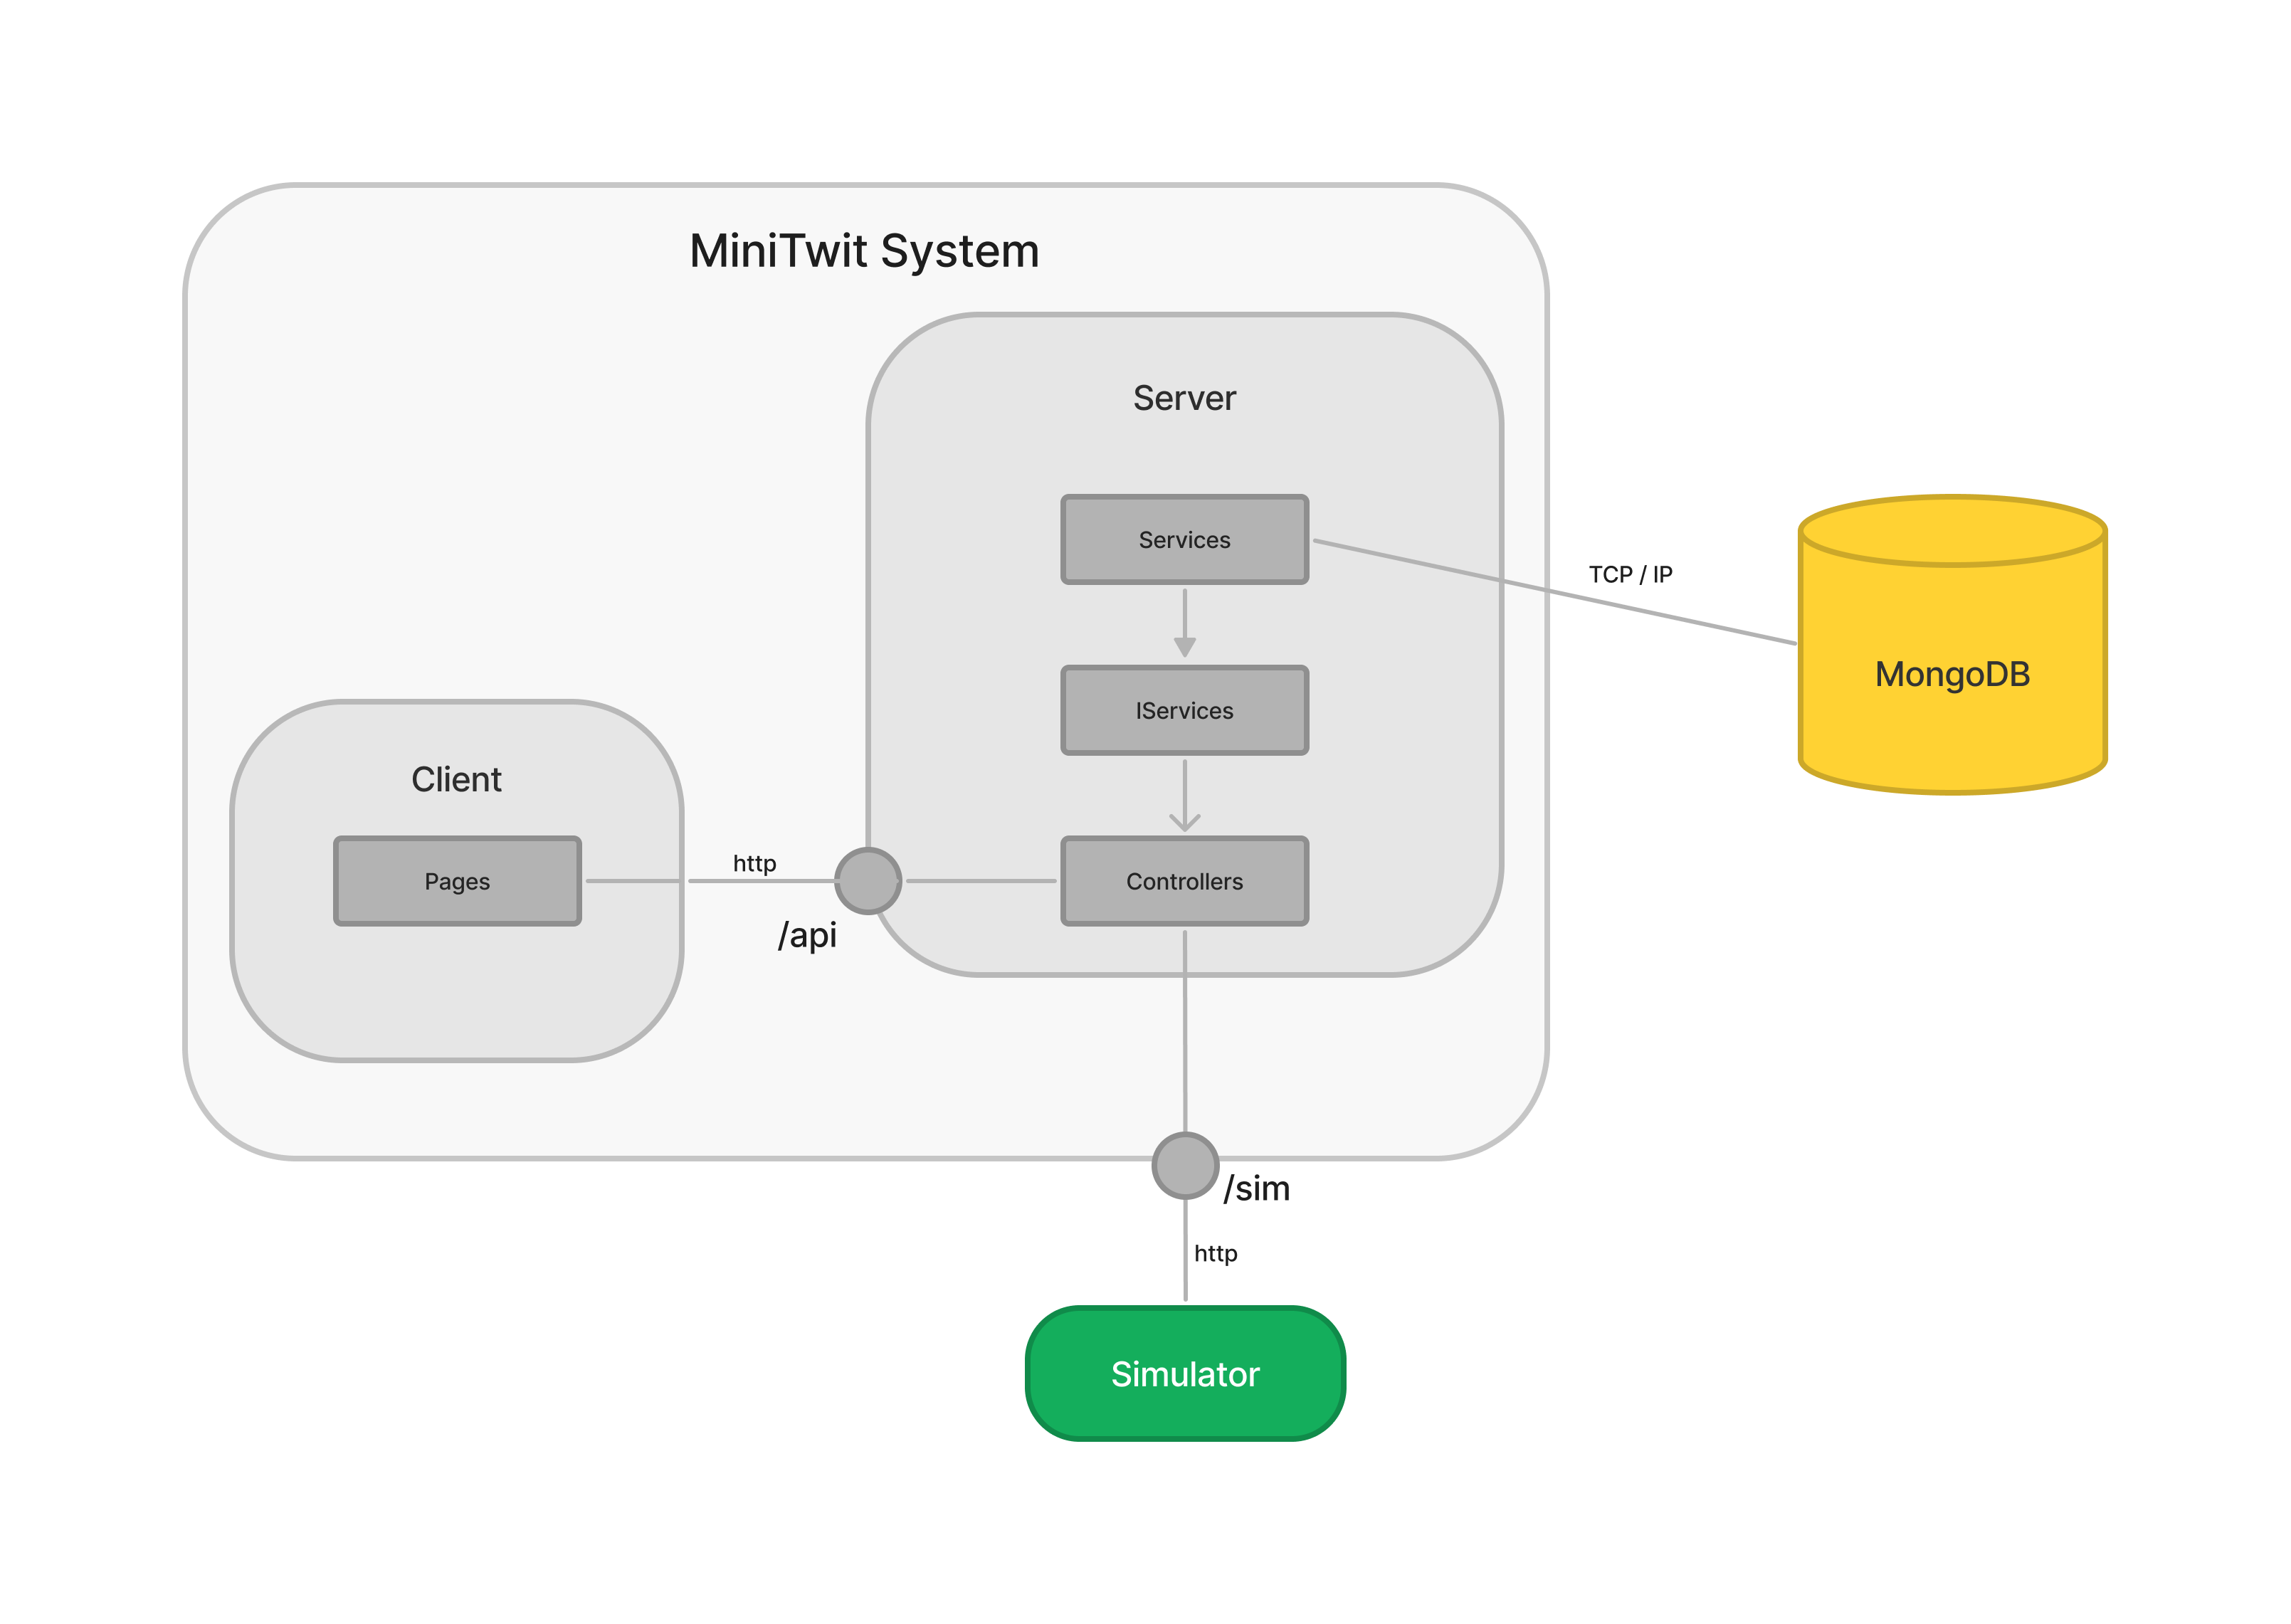
\includegraphics[width=14cm,height=12cm,keepaspectratio]{Diagrams/ComponentDiagram.png}
    \caption{Component diagram of the core system design.}
    \label{ComponentDiagram_1}
\end{figure}

Our system is split into two parts: \textit{Server} and \textit{Client}. The \textit{Server} is responsible for the backend part of the system, that is the business logic, exposing endpoints and interaction with the database. The \textit{Client} represents the frontend part of our system, and includes everything related to the user interface. %Maybe a rework on this last sentence, don't see the relevance here.

As for our database, we decided to use the \textit{NoSql} database \textit{MongoDB}. We found \textit{MongoDB} to be a fitting tool for the job as it goes nicely together with the idea of a cloud and scalable structure, which this whole project is based on. This also meant that we had the option of easily scaling our database in the future, should the need should arise. 
%We need some diagrams (Activity diagram, Class diagram, etc) Do not go into system architecture though

\subsection{System Architecture}

The system has a micro-service based architecture and is implemented by the use of docker containers. Our system is deployed on a \textit{Digital Ocean} Droplets\footnote{\url{https://www.digitalocean.com/products/droplets}} which is set up to run an \textit{Ubuntu} based virtual machine (VM). In total we have two VM's where several different applications runs, providing and supporting the \textit{MiniTwit} application.

We have defined a common sub-network\footnote{\url{https://docs.docker.com/compose/networking/}} inside the \textit{MiniTwit} VM, which includes all the containers there, enabling them to interact with each other. 

The database is located on a different \textit{Droplet} which excludes it from the common network mentioned in the section above. The reasoning behind placing the database on a separate \textit{Droplet} was a conscious effort in making the system more reliable and less prone to corruption of our live database. In case of a total system crash failure in our main Droplet, our data would still be intact in an other environment. However, as our deployment diagram\footnote{Figure \ref{DeploymentDiagram_1}} reflects we have not set up any redundant databases, which would further increase the reliability. An easier alternative to the redundancy approach, is the use of docker volumes\footnote{\url{https://docs.docker.com/storage/volumes/}}. This approach would ensure the data being persisted even though the container might crash, but would still be liable to failure if the whole VM were to shut down.

\begin{figure}[H]
    \centering
    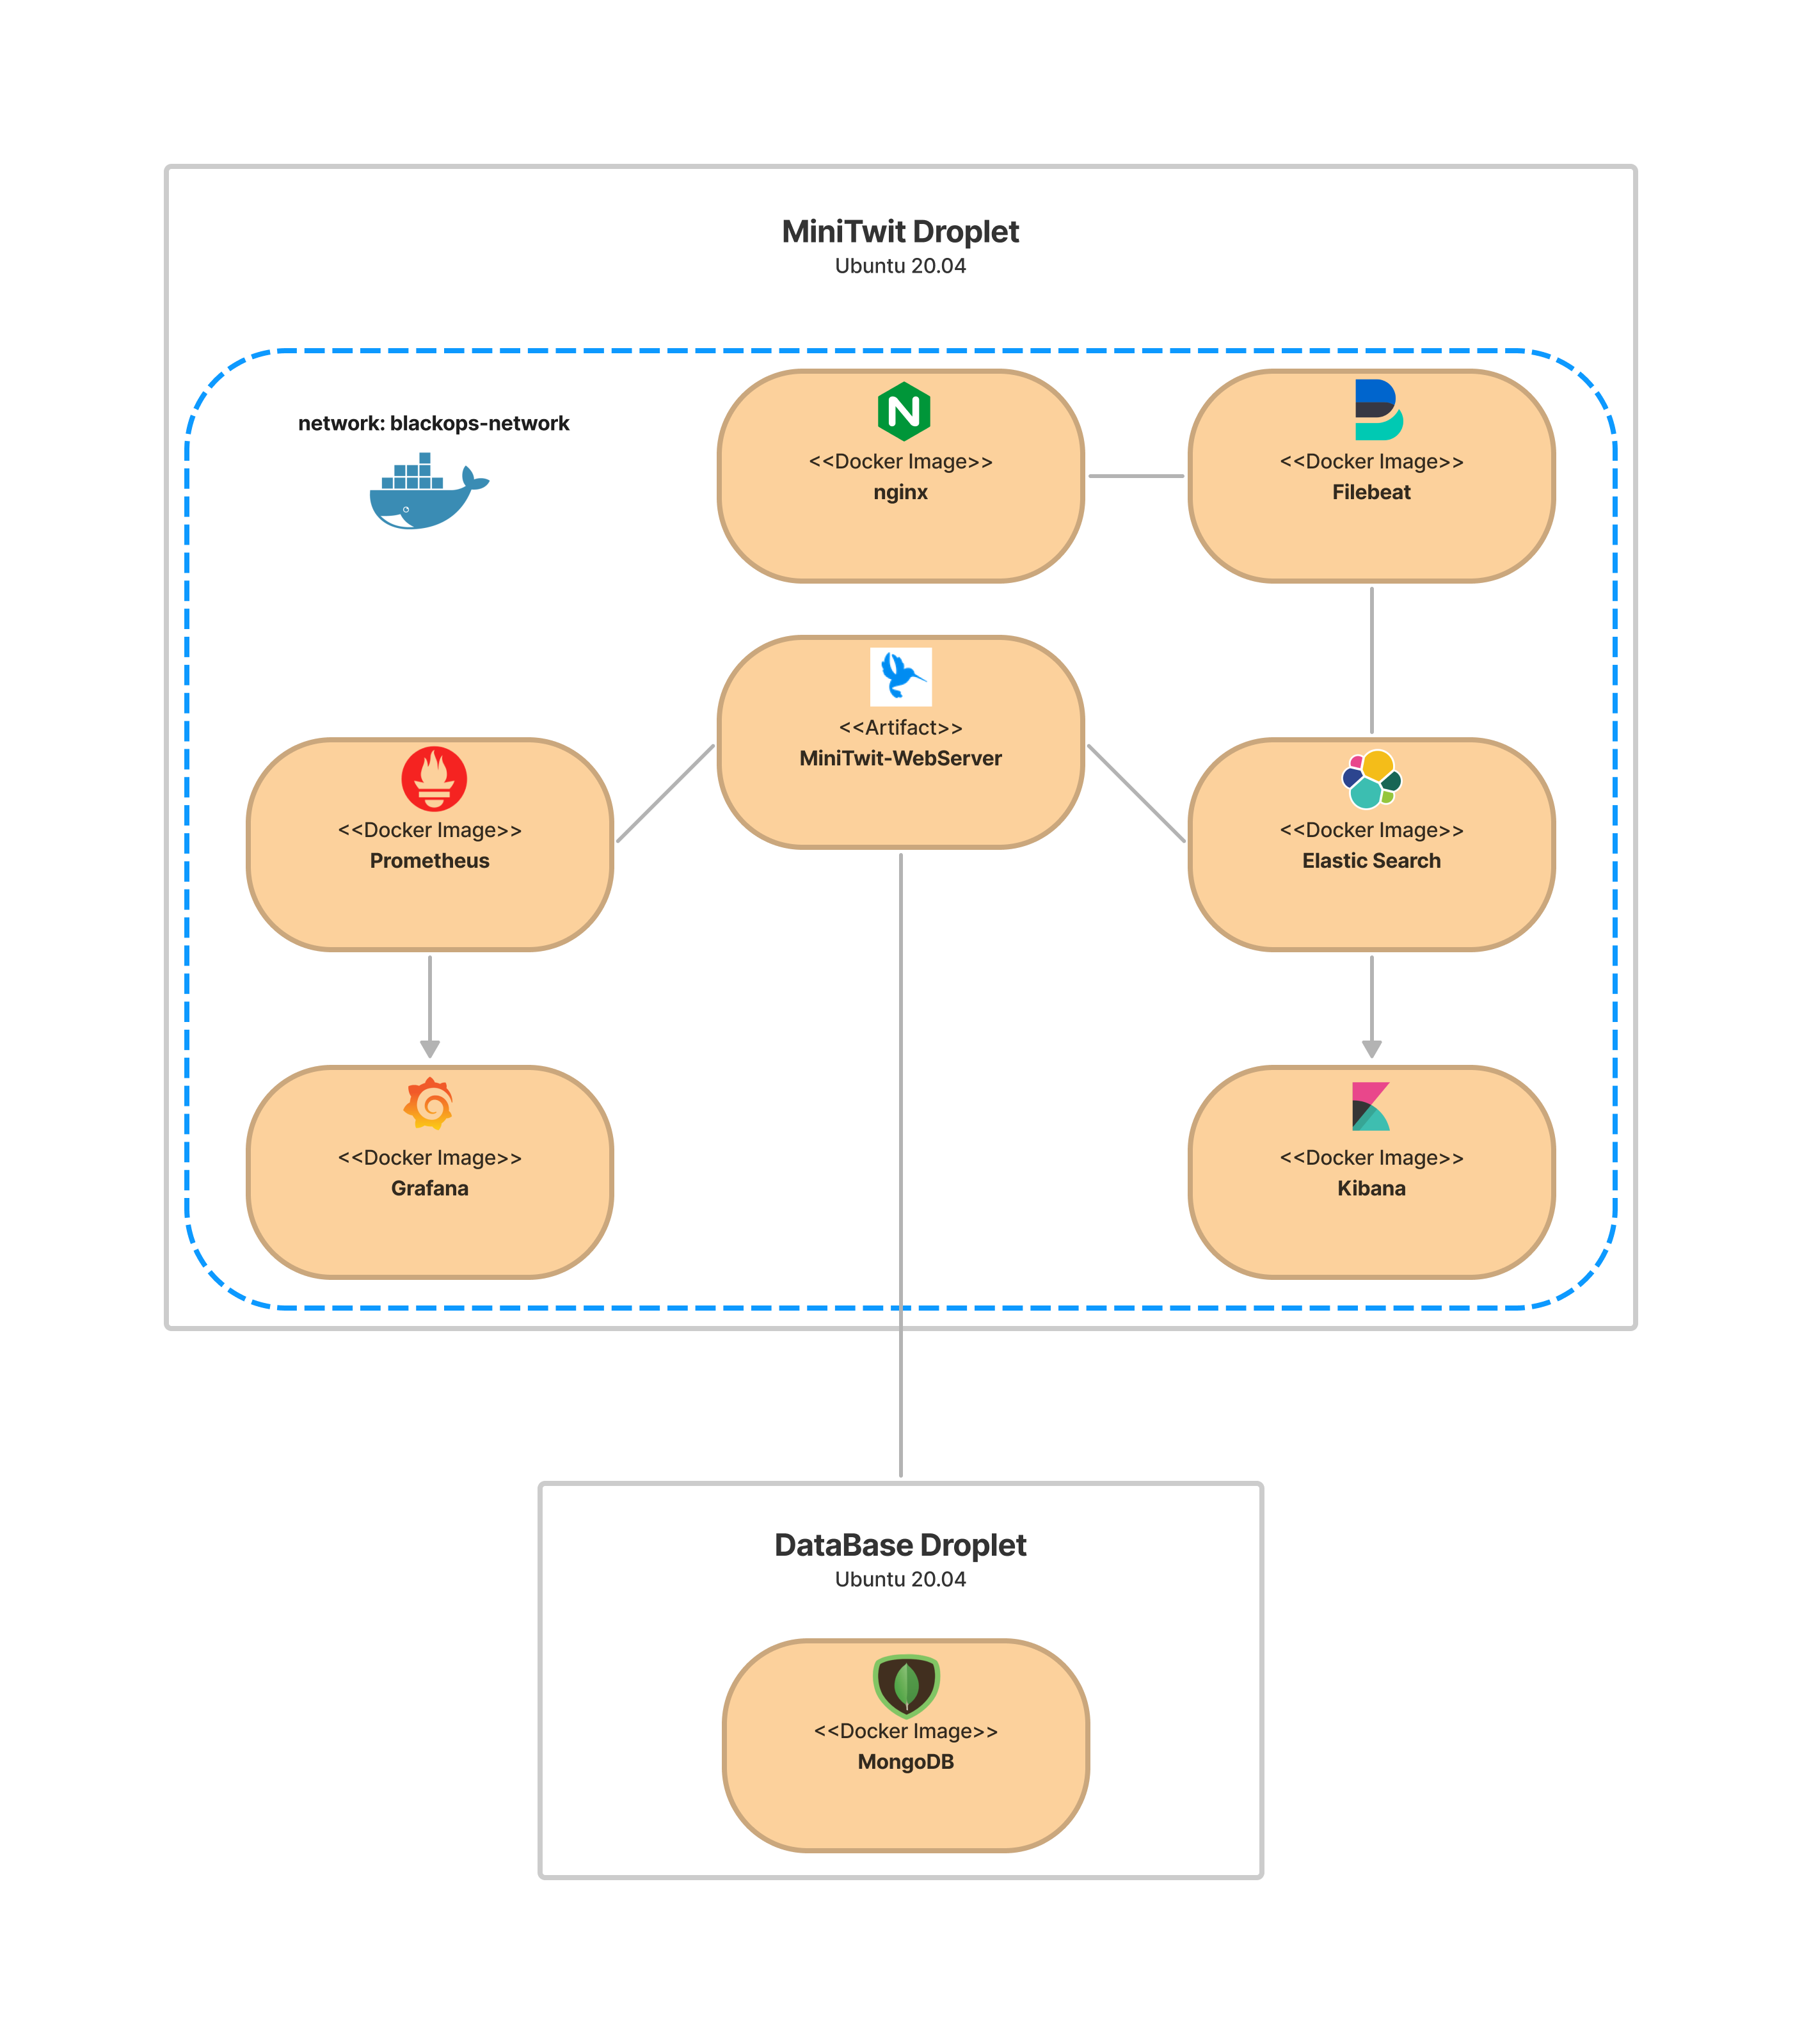
\includegraphics[width=14cm,height=12cm,keepaspectratio]{Diagrams/DevOpsDeploymentDiagram.png}
    \caption{Deployment diagram of the micro service based architecture.}
    \label{DeploymentDiagram_1}
\end{figure}

\subsubsection{Subsystems}
Our system is combined of many important subsystems that support and enable the \textit{MiniTwit} web application. The different subsystems all have very different purposes and together create a fully fledged system that allows for monitoring, logging, scalability and storage.

Even though most of the containers that the subsystems run in are instantiated in the same environment, they are not visible to each other by default. 

This realisation occurred to us when we instructed our \textit{Grafana} container to pull data from the Prometheus container on port :9090. Naturally, the container wasn't able to succeed as there was no receiver on the port in its sub network.

Many of the subsystems will be further elaborated upon later in the report in context to their area of responsibility.


% sequence diagrams 
% https://github.com/itu-devops/lecture_notes/blob/master/sessions/session_13/Architectural_Viewpoints.pdf

%INSERT SEQUENCE DIAGRAM 

%Digital ocean. Cloud development

%Go into subsystems that we use (but not into detail as they will be covered later (Grafana, Docker, Prometheus) (go into detail about MongoDB))

\subsection{System Dependencies}
A list of all direct technologies and tools we use in this project can be found in Appendix 7.5. For most parts we are using "static" versions, instead of latest version. Using the latest version ensures that the technology is up-to-date, however there is also the risk of newer versions not being able to work together. An example is, if a tool is updated so it uses a new API, then your system will fail. 

Making sure everything is running on the same version does however allow for an increase in stability amongst the technologies.

In the group we haven't really decided which way we prefer, but currently in the project we are leaning towards static version, which we can update as needed. 

\subsection{Current State}

The system in its current state contains some issues that preferably should be resolved. These are revealed by static code scanning tools.


\subsubsection{Test Coverage Percentage}
We prioritized implementing tests for the \textbf{MessagesController} and \textbf{UsersController} classes.

The test coverage of the entire system is 44\%, as seen in Figure 4. The server assembly has a test coverage of 30\%.\footnote{See appendix: Figure\_\ref{ServerAssembly}} Preferably, test coverage should be greatly expanded to cover more aspects of the application and exhaustively test all controller endpoints.

As it stands, controllers are tested independently using Mock data. We would benefit from using integration testing in addition to this, which would allow us to discover issues when the controllers retrieve real data.

\begin{figure}[H]
    \centering
    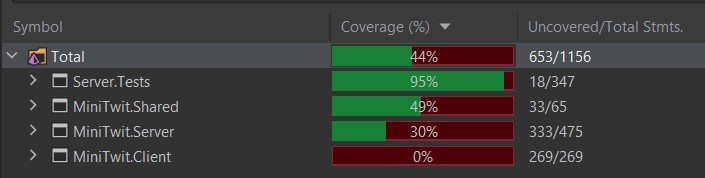
\includegraphics[width=16cm,height=14cm,keepaspectratio]{Diagrams/test coverage.jpg}
    \caption{Test coverage of Minitwit.}
    \label{ComponentDiagram_1}
\end{figure}

%Snyk report
\subsubsection{Snyk Report}
\textit{Snyk} is able to identify and highlight security vulnerabilities in dependencies, container images and infrastructure configurations. Here \textit{Snyk} has identified a series of vulnerabilities (see Figure 5), some of which are easily addressed. It is worth noting, that two issues of critical severity have been discovered. These are both instances of allowing remote code execution, by being dependent on a vulnerable version of the the library '\textit{System.Text.Encodings.Web}'. Preferably, this critical security issue should be addressed by updating to a newer version. 

\begin{figure}[H]
    \centering
    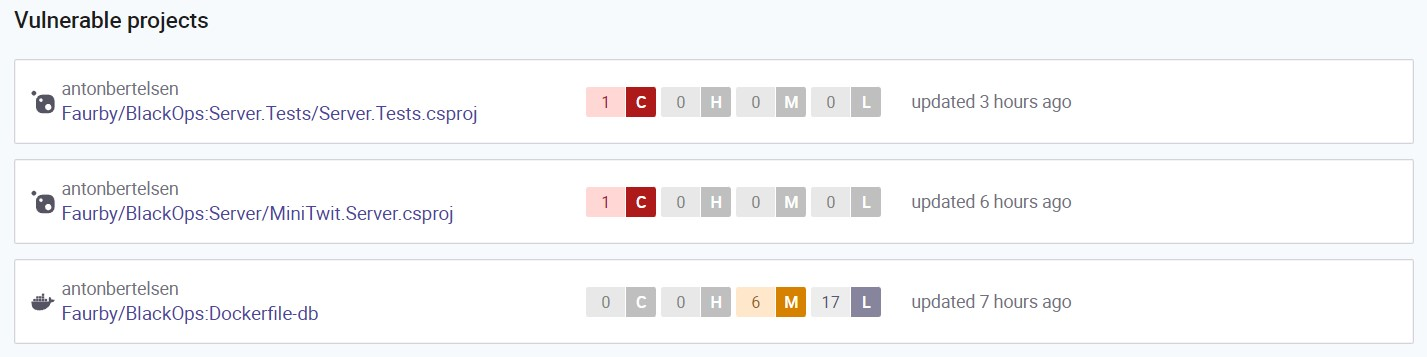
\includegraphics[width=16cm,height=14cm,keepaspectratio]{Diagrams/snyk.jpg}
    \caption{Snyk dashboard showing identified security issues.}
    \label{ComponentDiagram_1}
\end{figure}

%Sonarcloud report
\subsubsection{SonarCloud Report}
\textit{SonarCloud} automatically scans code and highlights opportunities to improve quality and security. In Figure 6, it is worth noting that 15 of the 22 identified issues relate to using razor specific CSS syntax that \textit{SonarCloud} is unfamiliar with and presumes to be a mistake.

\begin{figure}[H]
    \centering
    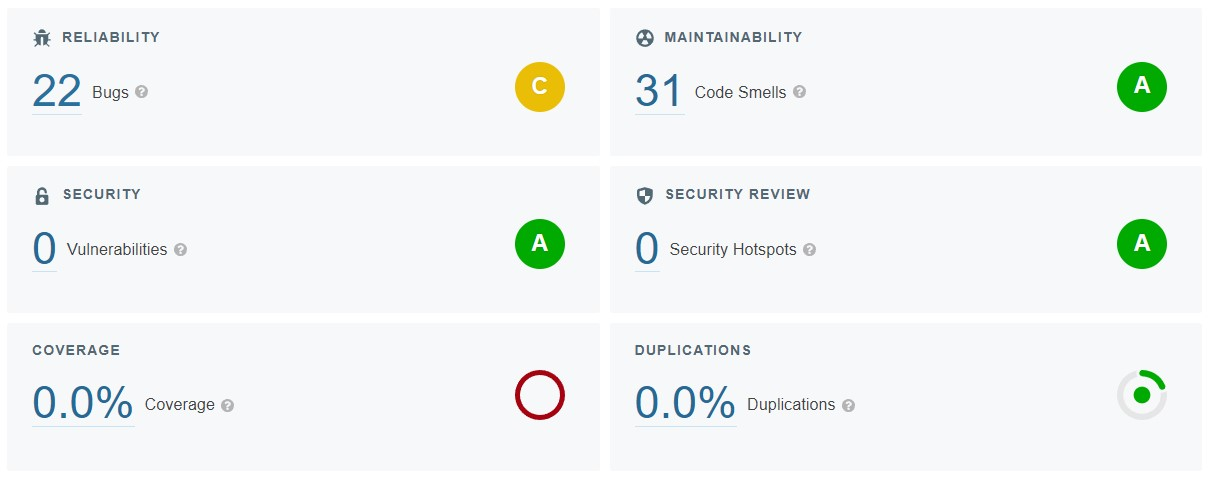
\includegraphics[width=16cm,height=14cm,keepaspectratio]{Diagrams/sonarcloud.jpg}
    \caption{SonarCloud dashboard showing identified bugs and code smells.}
    \label{ComponentDiagram_1}
\end{figure}

\subsubsection{Lighthouse Report}
\textit{Lighthouse} rates the page on a series of performance factors to give it an overall performance score. In Figure 7, \textit{Minitwit} receives a score of 43, which shows there is much room for improvement. One reason that the page is slow to start is that we use \textit{Blazor} Web assembly, which requires a large amount of data to be sent to the client when they first connect to the page.

\begin{figure}[H]
    \centering
    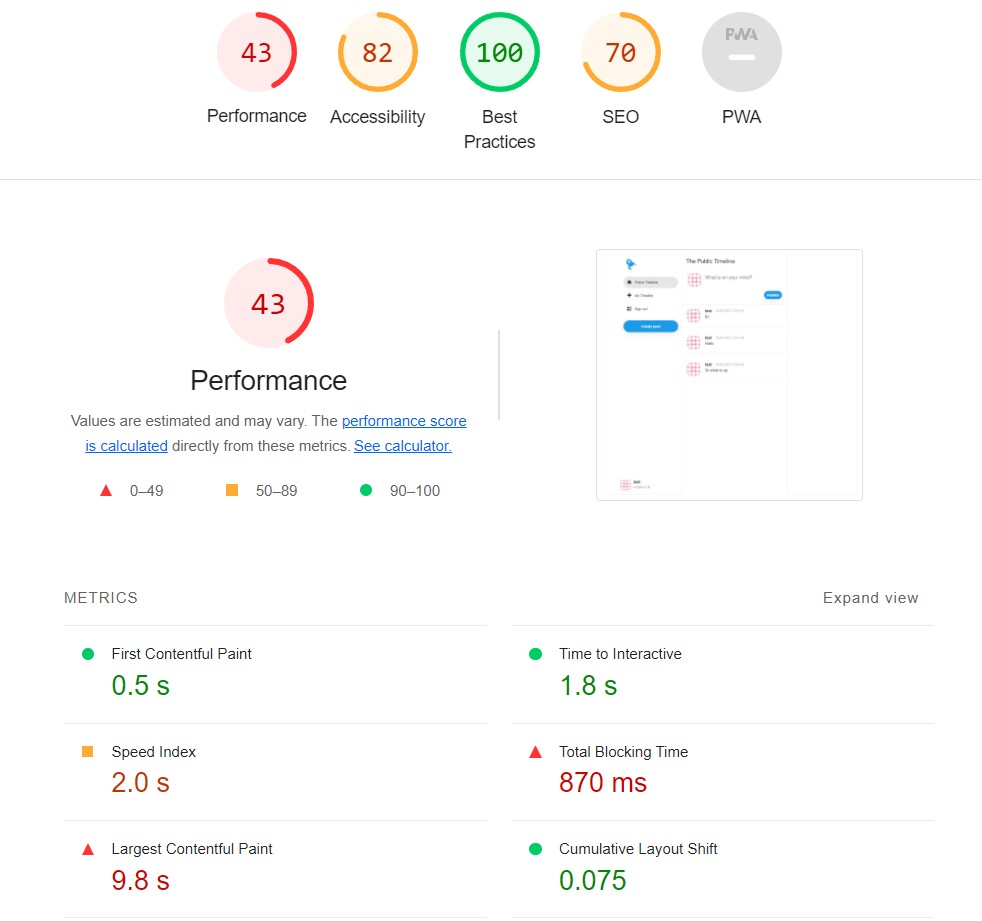
\includegraphics[width=16cm,height=14cm,keepaspectratio]{Diagrams/lighthouse.jpg}
    \caption{Lighthouse report showing page performance.}
    \label{ComponentDiagram_1}
\end{figure}


\subsection{License compatibility}
We are using the \textit{MIT} license, which from this source\footnote{\url{https://dwheeler.com/essays/floss-license-slide.html}} says it is compatible with the rest of the open source dependencies. However some dependencies like \textit{ASP NET Core} have their own \textit{Microsoft} license, so they are not open source.

We know that the \textit{MIT} license is the most popular license on \textit{GitHub}.\footnote{\url{https://github.blog/2015-03-09-open-source-license-usage-on-github-com/}}

Figure \ref{fig:scancodelicenses} shows how the dependencies in our project are primarily MIT licensed, and open source.

\begin{figure}[H]
    \centering
    \includegraphics[width=16cm, keepaspectratio]{Diagrams/Scancode-licenses2.png}
    \caption{ScanCode licenses visualized}
    \label{fig:scancodelicenses}
\end{figure}
